\documentclass[11pt]{article}

\usepackage[T1]{fontenc}
\usepackage[utf8]{inputenc}
\usepackage[margin=1in]{geometry}
\usepackage{mathpazo}
\usepackage{microtype}
\usepackage{xcolor}
\usepackage{graphicx}
\usepackage{booktabs}
\usepackage{tabularx}
\usepackage{array}
\usepackage{float}
\usepackage{caption}
\usepackage{enumitem}
\usepackage{hyperref}

\definecolor{ink}{HTML}{102A43}
\definecolor{accent}{HTML}{1F4E79}
\definecolor{warm}{HTML}{B04A2F}
\definecolor{muted}{HTML}{52606D}
\definecolor{panel}{HTML}{F7F5EF}
\definecolor{panelborder}{HTML}{D9E2EC}

\hypersetup{
  colorlinks=true,
  linkcolor=accent,
  citecolor=accent,
  urlcolor=accent,
  pdftitle={Structured Yet Fragile: Signed Intervention Geometry of Matched ORF and CRISPR Cell Painting Profiles},
  pdfauthor={Ali Uyar}
}
\urlstyle{same}

\setlength{\parindent}{0pt}
\setlength{\parskip}{0.6em}
\renewcommand{\arraystretch}{1.15}
\graphicspath{{figures/}}

\newcommand{\panelbox}[1]{%
  \begingroup
  \setlength{\fboxsep}{10pt}%
  \noindent\colorbox{panel}{%
    \parbox{\dimexpr\textwidth-2\fboxsep\relax}{#1}%
  }%
  \endgroup
}

\begin{document}

\pagenumbering{gobble}
\begin{titlepage}
\color{ink}
\vspace*{1.5cm}

{\Large\bfseries Structured Yet Fragile:\\[0.25em]
Signed Intervention Geometry of Matched ORF and CRISPR Cell Painting Profiles\par}

\vspace{1.0cm}

{\large Ali Uyar\par}
{\normalsize Independent Researcher\par}

\vspace{0.8cm}

{\small
Official locked run: \texttt{offv1\_\_featint\_\_platectrl\_\_thrA2\_thrR2\_\_z1p96\_\_beta1p0}\\
Analysis date: 23 March 2026
\par}

\vspace{1.0cm}
\hrule
\vspace{0.6cm}

\textbf{Overview.}
This manuscript reports a locked analysis of same-gene ORF and CRISPR Cell Painting profiles. The central result is not a clean, robust signed geometry law, but a biologically organized regime map that is dominated by asymmetric and ambiguous states, only partially stable across preprocessing variants, and too weak to support a strong retrieval-style utility claim.

\vfill

\textbf{Keywords:} Cell Painting; morphological profiling; ORF; CRISPR; perturbation biology; robustness; negative result; preprocessing fragility
\end{titlepage}

\color{ink}
\clearpage
\pagenumbering{arabic}

\section*{Abstract}
Matched gain- and loss-of-function perturbations are an attractive setting in which to ask whether cellular morphology occupies a signed regime space with interpretable axes such as alignment, inversion, orthogonality, and modality-specific asymmetry. We tested that question in a locked, auditable pipeline on the \texttt{cpg0016} subset of the JUMP Cell Painting genetic resource, focusing on same-gene ORF and CRISPR pairs. Across 5,332 analyzed gene pairs, 2,552 were active in both modalities and 2,724 received confident non-inactive labels after bootstrap consensus. The resulting landscape was structured but not cleanly symmetric: 48.9\% of pairs were labeled ambiguous, 30.3\% asymmetric\_CRISPR, 20.8\% asymmetric\_ORF, and only 3 genes inactive; no aligned, inverse, or orthogonal labels survived the final consensus layer. Robustness was mixed rather than absent. Agreement was high under no-final-centering (0.951 primary-only agreement) and very high under the dedicated artifact-sensitivity comparison (0.994), but only moderate under the interpretable pipeline (0.758), and regime prevalence shifted strongly across mean-strength deciles (maximum absolute fraction shift 0.434). Biological signal remained detectable despite this fragility, with 536 significant Reactome terms concentrated in asymmetric regimes, whereas retrieval remained effectively null-like and did not support a useful regime-aware ranking claim. The locked evidence therefore supports a restrained but non-null conclusion: same-gene ORF and CRISPR morphology occupies a biologically meaningful regime map, yet that map is dominated by asymmetry, preprocessing dependence, and fragility rather than by a robust symmetric signed geometry.

\panelbox{\textbf{Main claim.} Under a locked, auditable analysis of same-gene ORF and CRISPR Cell Painting profiles, signed intervention geometry is \emph{structured yet fragile}: biological organization is visible, but the resulting map is dominated by asymmetric and ambiguous regimes and is not strong enough to support a robust retrieval-style positive claim.}

\section{Introduction}
Image-based profiling has become a powerful way to characterize perturbation effects at scale, with the Cell Painting assay providing a dense, reusable morphological representation of cell state \cite{bray2016cellpainting, cimini2023optimizing}. The JUMP Cell Painting Consortium extended this idea into a large public compendium of genetic and chemical perturbations, creating an opportunity to compare matched gain- and loss-of-function perturbations in a single feature space \cite{jump2025genetic}. The conceptual appeal is obvious: if ORF and CRISPR perturbations for the same gene occupy a meaningful signed relationship, then same-gene pairs might align, invert, decouple, or reveal systematic asymmetry that reflects dosage, compensation, or assay-specific biology.

That hypothesis is easy to oversell. Morphological profiling is exquisitely sensitive to preprocessing choices, replicate structure, feature-space alignment, and nuisance variation \cite{chandrasekaran2021upgrade, way2022complementary}. For this reason, the present study intentionally privileges auditable discipline over optimistic flexibility. We locked the analysis stack, validated checkpointed outputs, and interpreted the final manuscript strictly through the evidence bundle produced by the official run and three predefined robustness comparisons.

This design changes the inferential question. Rather than asking whether a tunable pipeline can be made to produce a favorable geometry story, we ask what survives when the methods are fixed in advance and evaluated against explicit robustness criteria. The answer is more constrained than the original positive hypothesis. A genuine regime structure exists, but it is overwhelmingly asymmetric and ambiguous, only partially stable across preprocessing choices, biologically interpretable in limited ways, and not retrieval-useful. That combination is scientifically valuable because it defines what a locked morphology pipeline can and cannot support.

\section{Study Design and Locked Analysis}
We analyzed the \texttt{cpg0016} genetic subset of JUMP Cell Painting, restricting attention to same-gene ORF and CRISPR pairs with sufficient retained-well support after centering and filtering. The official run analyzed 5,332 same-gene pairs. Profiles were plate-centered using negative controls, intersected in a shared feature space, and summarized into per-gene modality statistics. Activity and reproducibility thresholds were locked at a strength z-score of 2.0 and a replicate-consistency z-score of 2.0, with at least two treated wells required per gene-modality.

Signed geometry was computed from matched ORF and CRISPR gene centroids using a signed cosine framework with activity-aware nulls. Regime assignment used a sign z-threshold of 1.96, an asymmetry threshold of 1.0, 200 bootstrap samples, and a 0.7 consensus threshold. The robustness stack comprised within-run confound checks (magnitude residualization, leave-one-plate-out stability, cell-count availability scan, strength-decile prevalence shift, and artifact sensitivity) together with three locked comparison runs: an interpretable pipeline, a no-final-centering pipeline, and an explicit artifact-sensitivity pipeline.

\begin{table}[H]
\centering
\caption{\textbf{Core quantitative summary of the locked official run.} These quantities define the strongest interpretation supported by the completed evidence bundle.}
\begin{tabularx}{\textwidth}{>{\raggedright\arraybackslash}p{0.55\textwidth} >{\raggedleft\arraybackslash}X}
\toprule
Metric & Value \\
\midrule
Analyzed same-gene ORF/CRISPR pairs & 5,332 \\
Pairs active in both modalities & 2,552 \\
Confident non-inactive final labels & 2,724 \\
Final ambiguous fraction & 48.9\% \\
Final asymmetric\_CRISPR fraction & 30.3\% \\
Final asymmetric\_ORF fraction & 20.8\% \\
Plate-holdout final-label agreement & 0.868 \\
Artifact-removal final-label agreement & 0.896 \\
Official vs. interpretable primary-only agreement & 0.758 \\
Official vs. no-final-centering primary-only agreement & 0.951 \\
Official vs. artifact-sensitivity primary-only agreement & 0.994 \\
Best official retrieval MRR (primary score) & 0.001656 \\
Significant Reactome terms & 536 \\
Significant CORUM terms & 0 \\
\bottomrule
\end{tabularx}
\end{table}

\section{Results}

\subsection{A regime map exists, but it is dominated by asymmetry and ambiguity}
The official run supports the existence of a same-gene morphological regime map, but not the one originally hoped for. The final regime distribution is strikingly concentrated in ambiguous and asymmetric labels: 2,605 genes were ambiguous, 1,613 asymmetric\_CRISPR, 1,111 asymmetric\_ORF, and only 3 inactive. No aligned, inverse, or orthogonal labels survived the final bootstrap-consensus stage. In other words, the data do not support a clean taxonomy in which gain- and loss-of-function perturbations typically behave as strong signed opposites. Instead, the dominant motif is that one modality tends to express a stronger or more stable morphological effect than the other.

This point matters for framing. The existence of structure alone is not enough to justify a positive discovery claim. What the official geometry actually says is that matched ORF and CRISPR perturbations occupy a constrained but highly skewed landscape. The map is therefore scientifically interesting, but not for the original reason. Its main message is asymmetry, not elegant bidirectional geometry.

\begin{figure}[H]
\centering
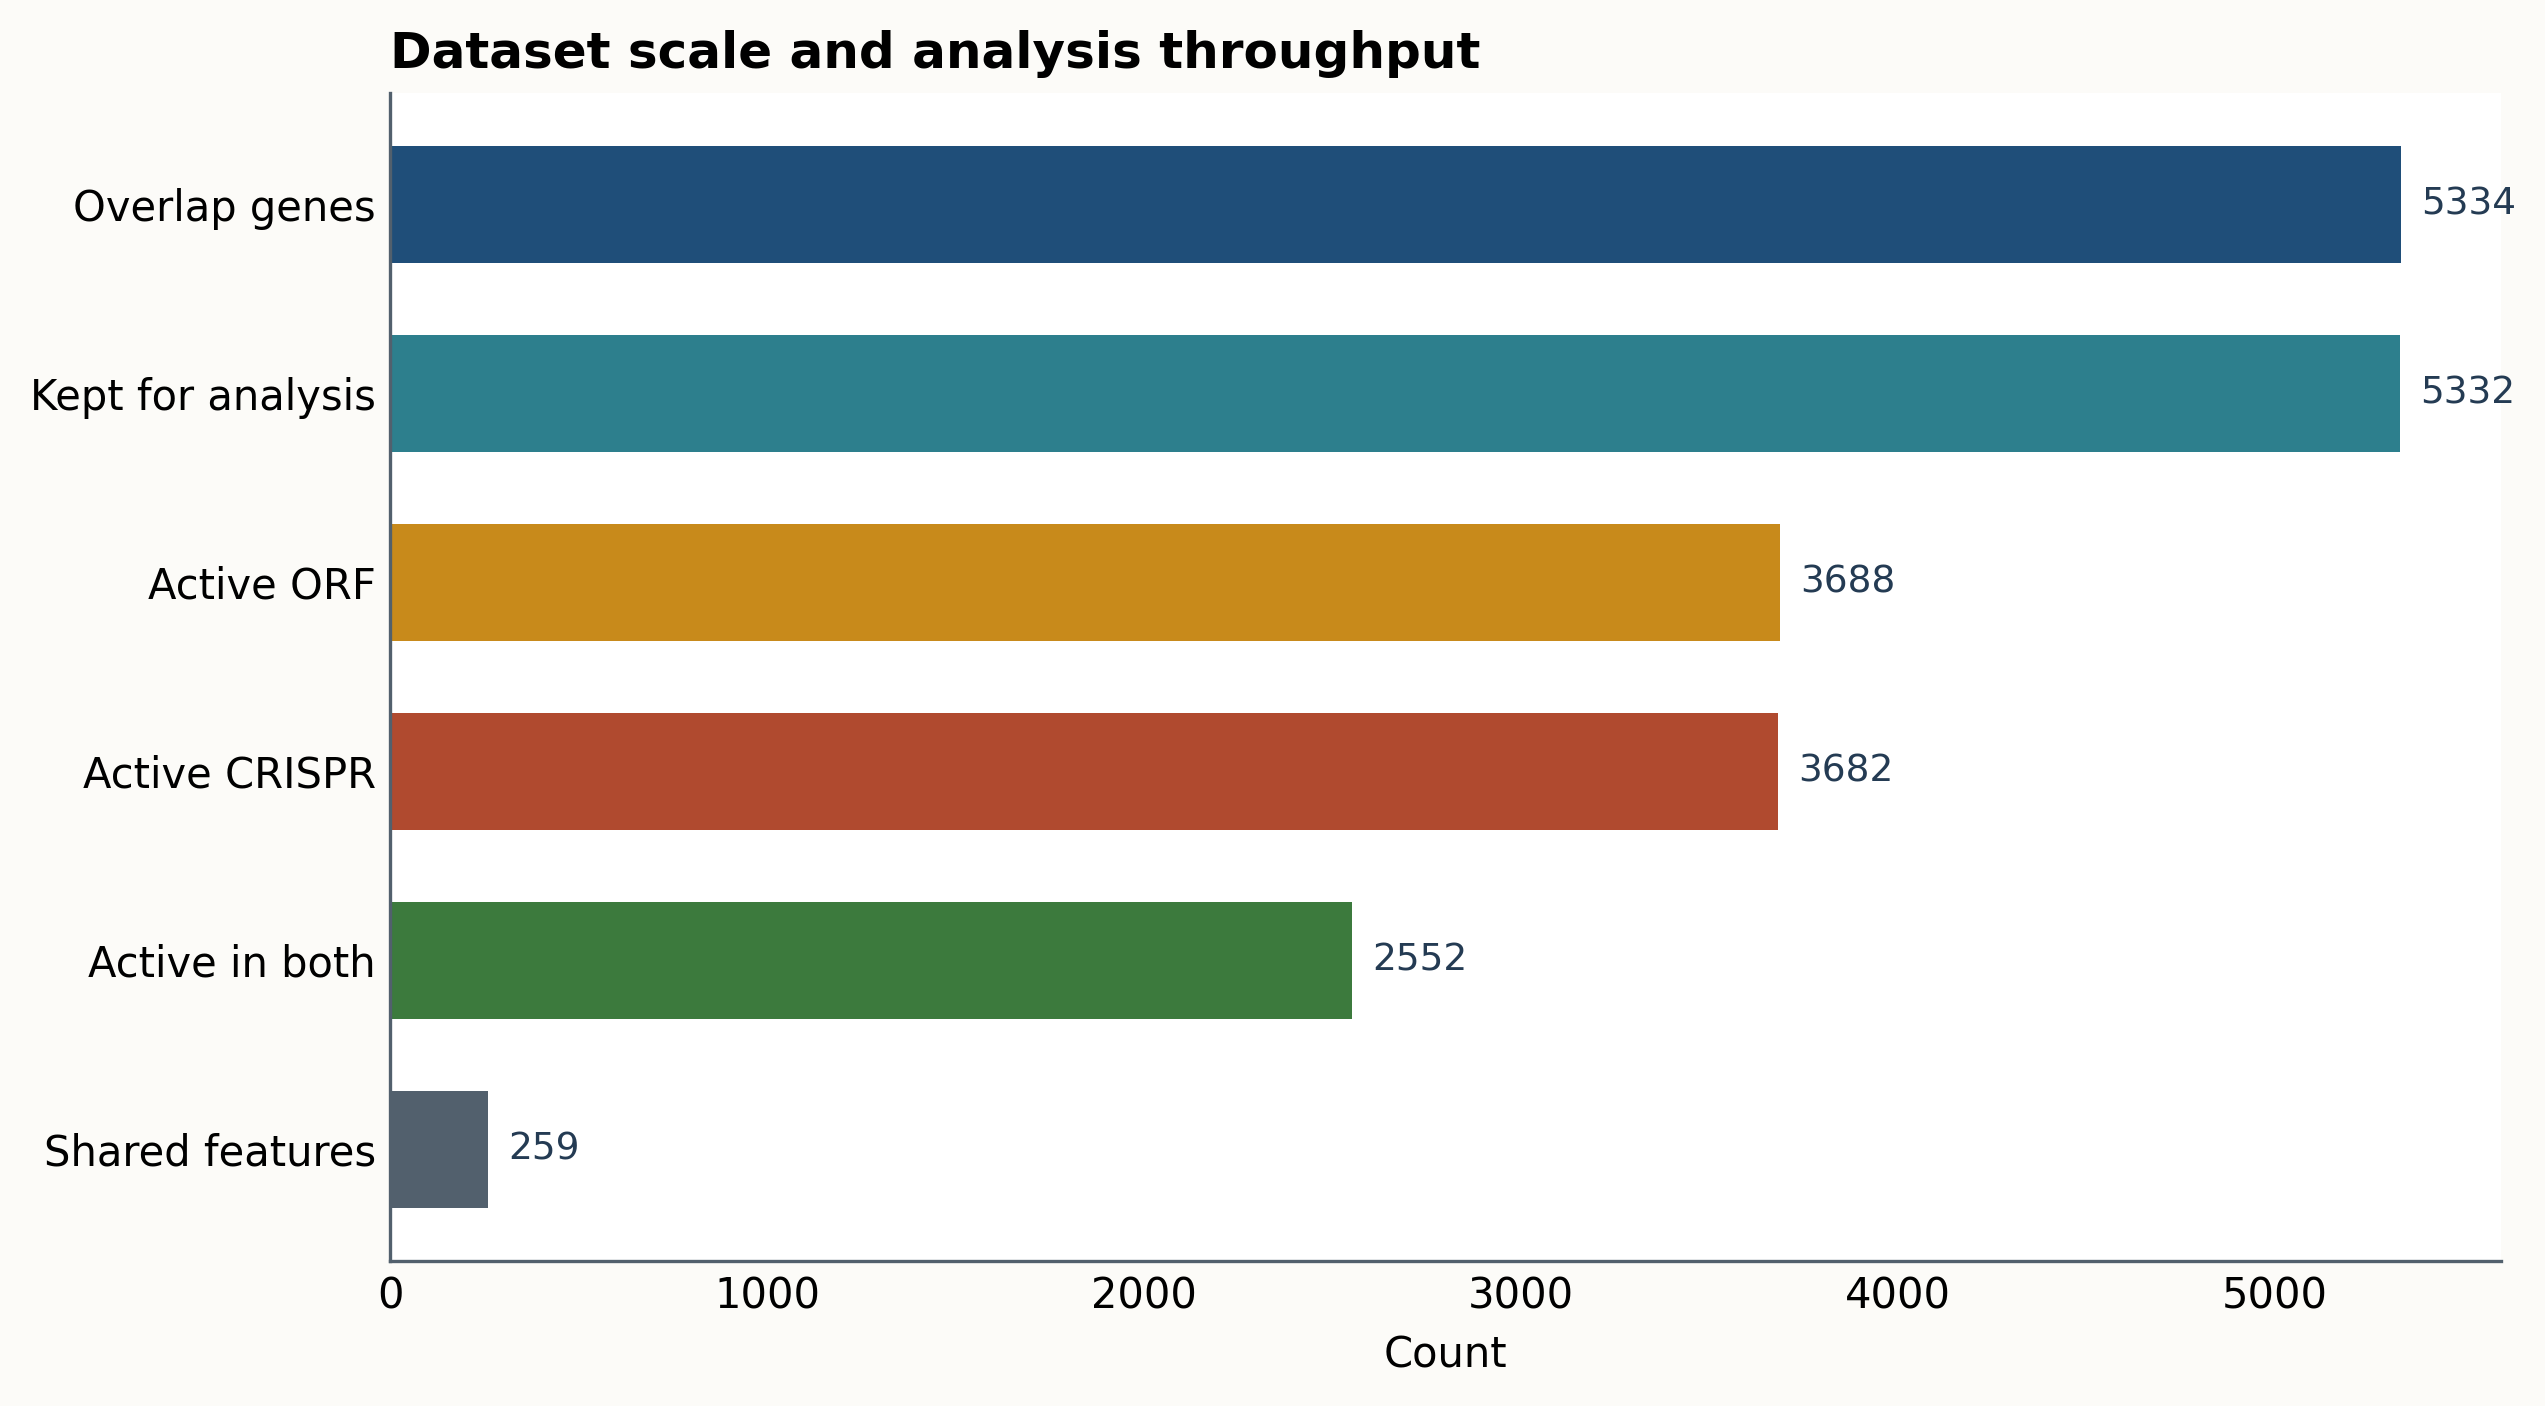
\includegraphics[width=0.93\textwidth]{figure1_dataset.png}
\caption{\textbf{Dataset scale and analysis throughput.} The locked pipeline retained a large enough subset of same-gene pairs to support structured inference, but downstream claims still depend on what kind of structure survives robustness checks.}
\end{figure}

\begin{figure}[H]
\centering
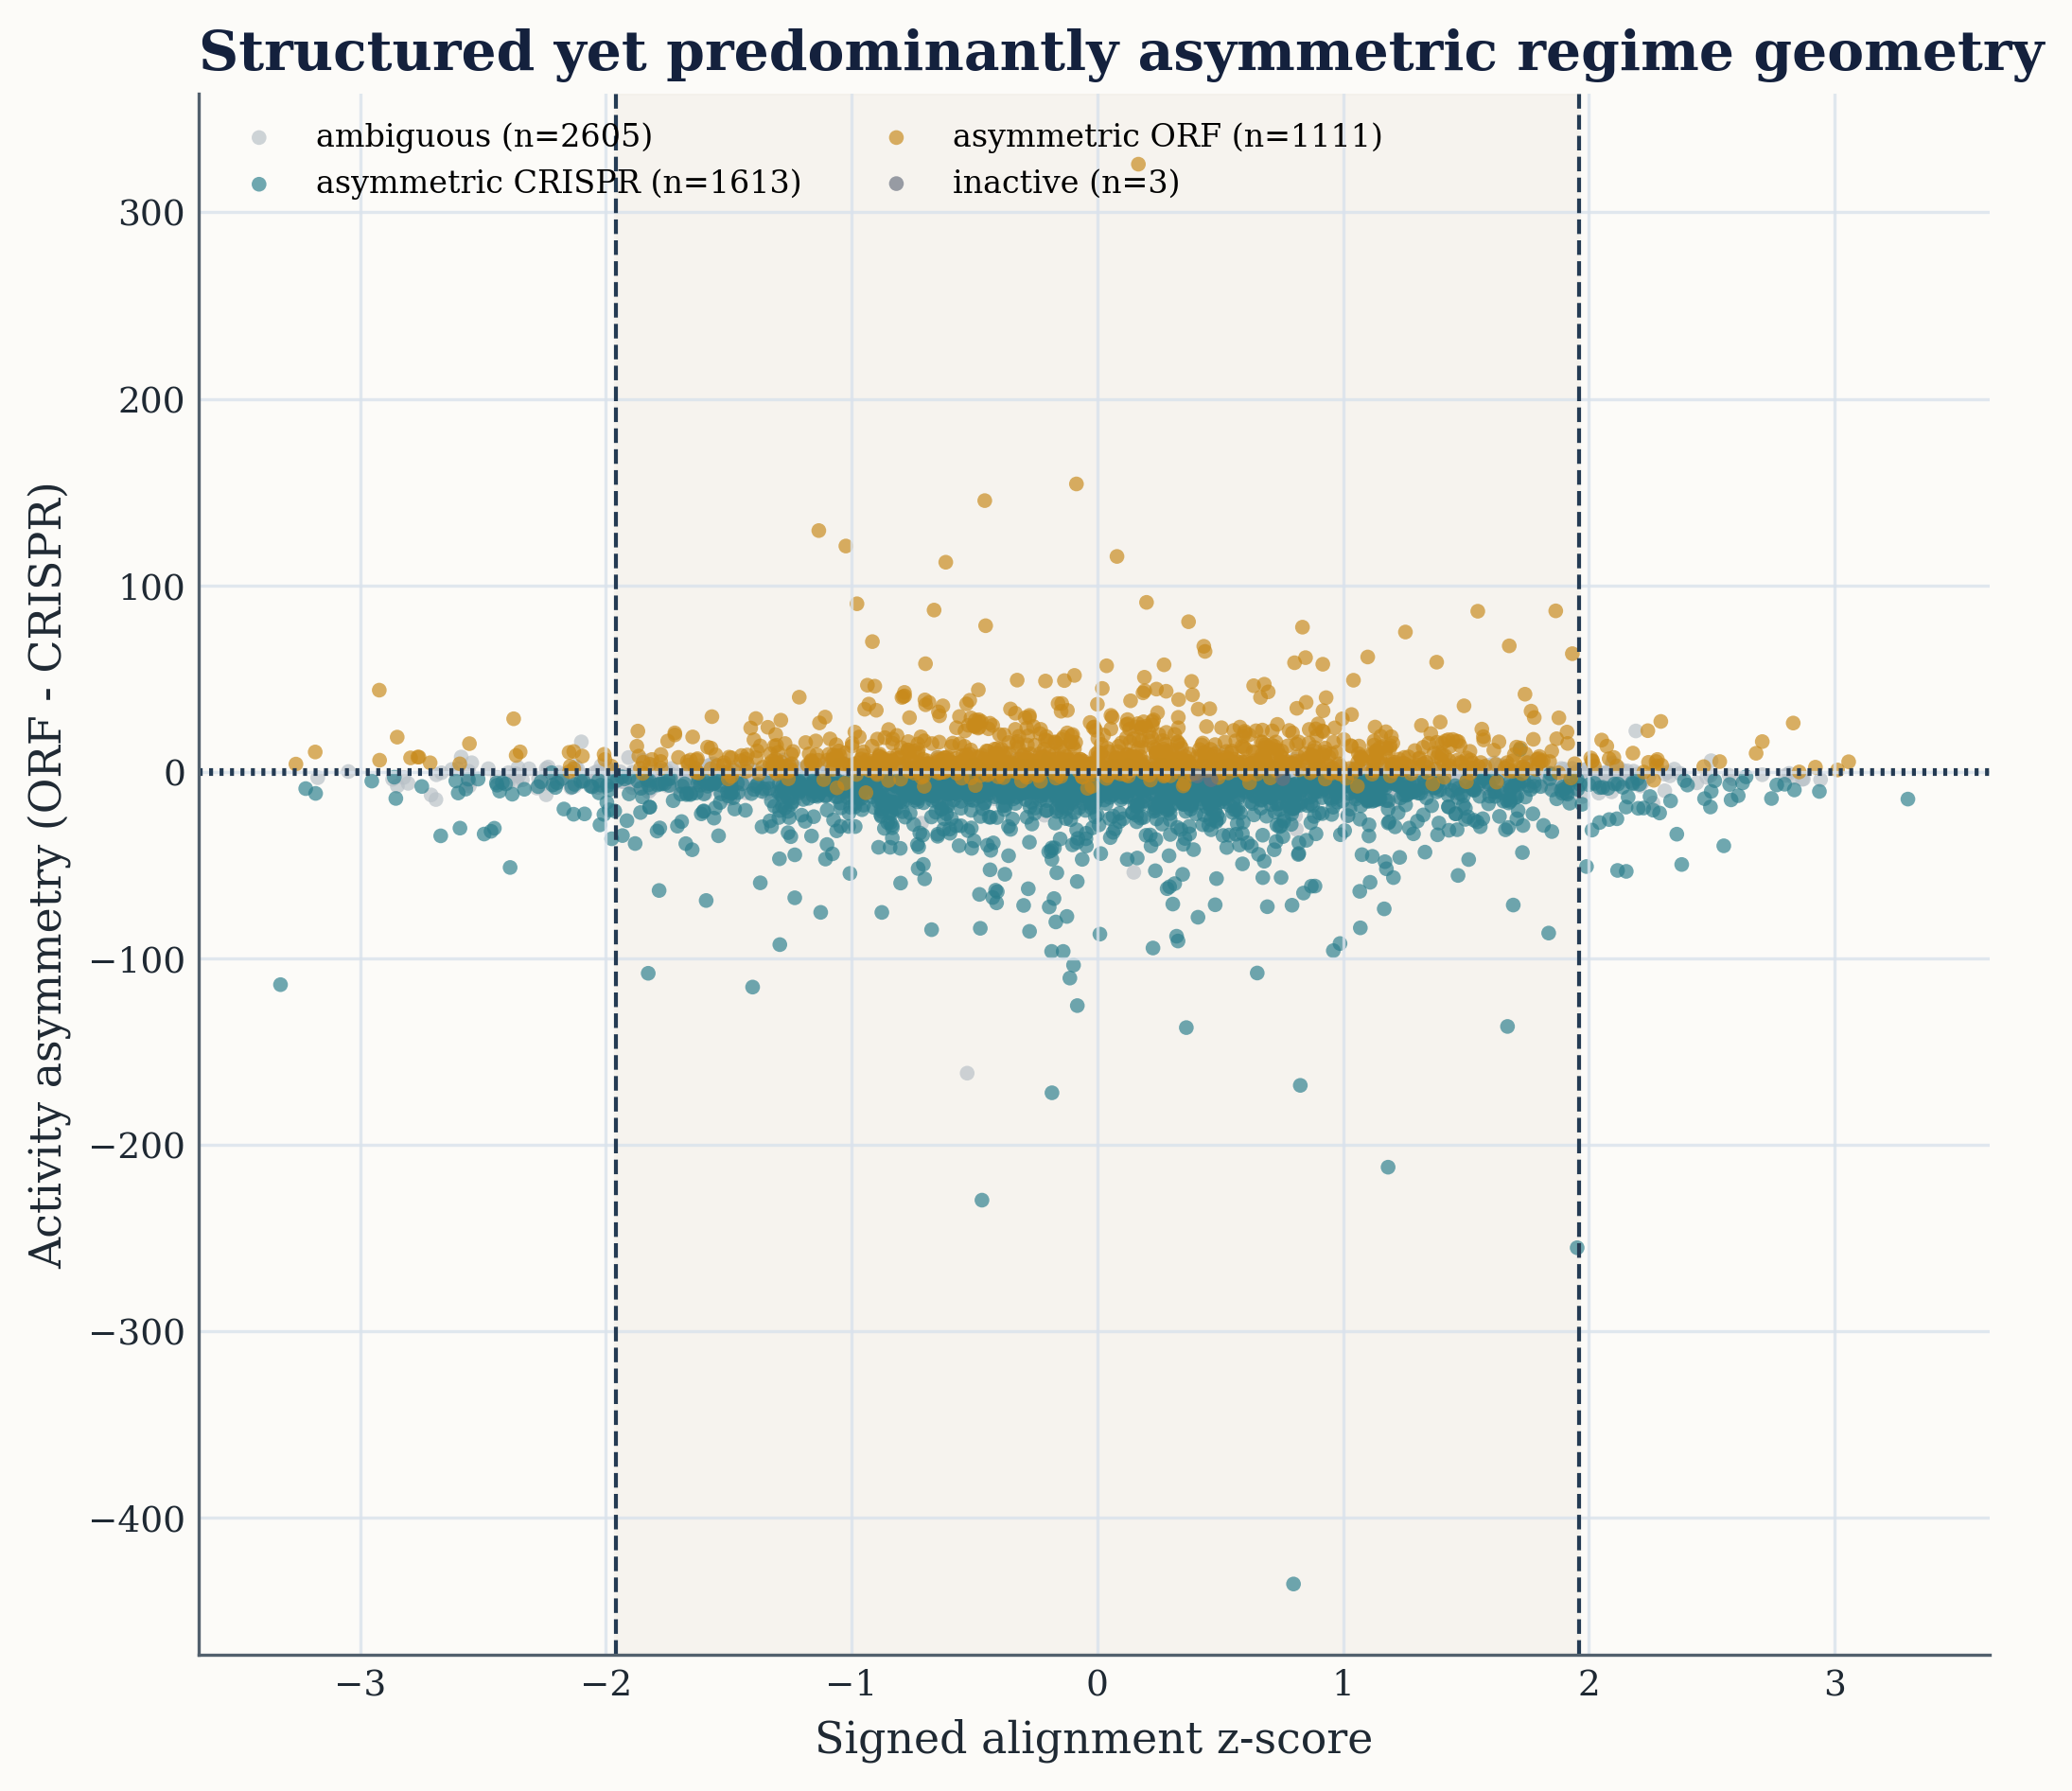
\includegraphics[width=0.93\textwidth]{figure2_regime_map.png}
\caption{\textbf{Signed intervention geometry is structured yet overwhelmingly asymmetric.} The decisive visual result is not the presence of strong aligned or inverse quadrants, but the dominance of ambiguous and asymmetric labels after bootstrap consensus.}
\end{figure}

\subsection{Robustness is partial: stable to some perturbations, fragile to others}
The most important result of the paper is not whether any signal exists, but how that signal behaves under locked robustness checks. On the encouraging side, the within-run plate-holdout agreement was 0.868, and the artifact-removal agreement was 0.896. Cross-run agreement was also very high for no-final-centering (0.951 primary-only agreement) and for the dedicated artifact-sensitivity comparison (0.994). These are not the numbers of a completely unstable pipeline.

However, the story does not remain positive once all checks are considered jointly. The interpretable pipeline reached only moderate agreement with the official run (0.758 primary-only agreement), and the strongest confound signal was unfavorable: regime prevalence shifted across mean-strength deciles with a maximum absolute fraction shift of 0.434. That specific failure matters because it suggests that part of the apparent regime composition is entangled with effect magnitude rather than reflecting a clean, preprocessing-invariant biological geometry.

This is why the final release report labels the project a \emph{pivot} rather than a positive release. The signal survives several reasonable perturbations of the analysis, but not enough of them, and not in the right way, to justify the original strong claim. The correct interpretation is therefore \emph{partial stability with explicit fragility}.

\begin{figure}[H]
\centering
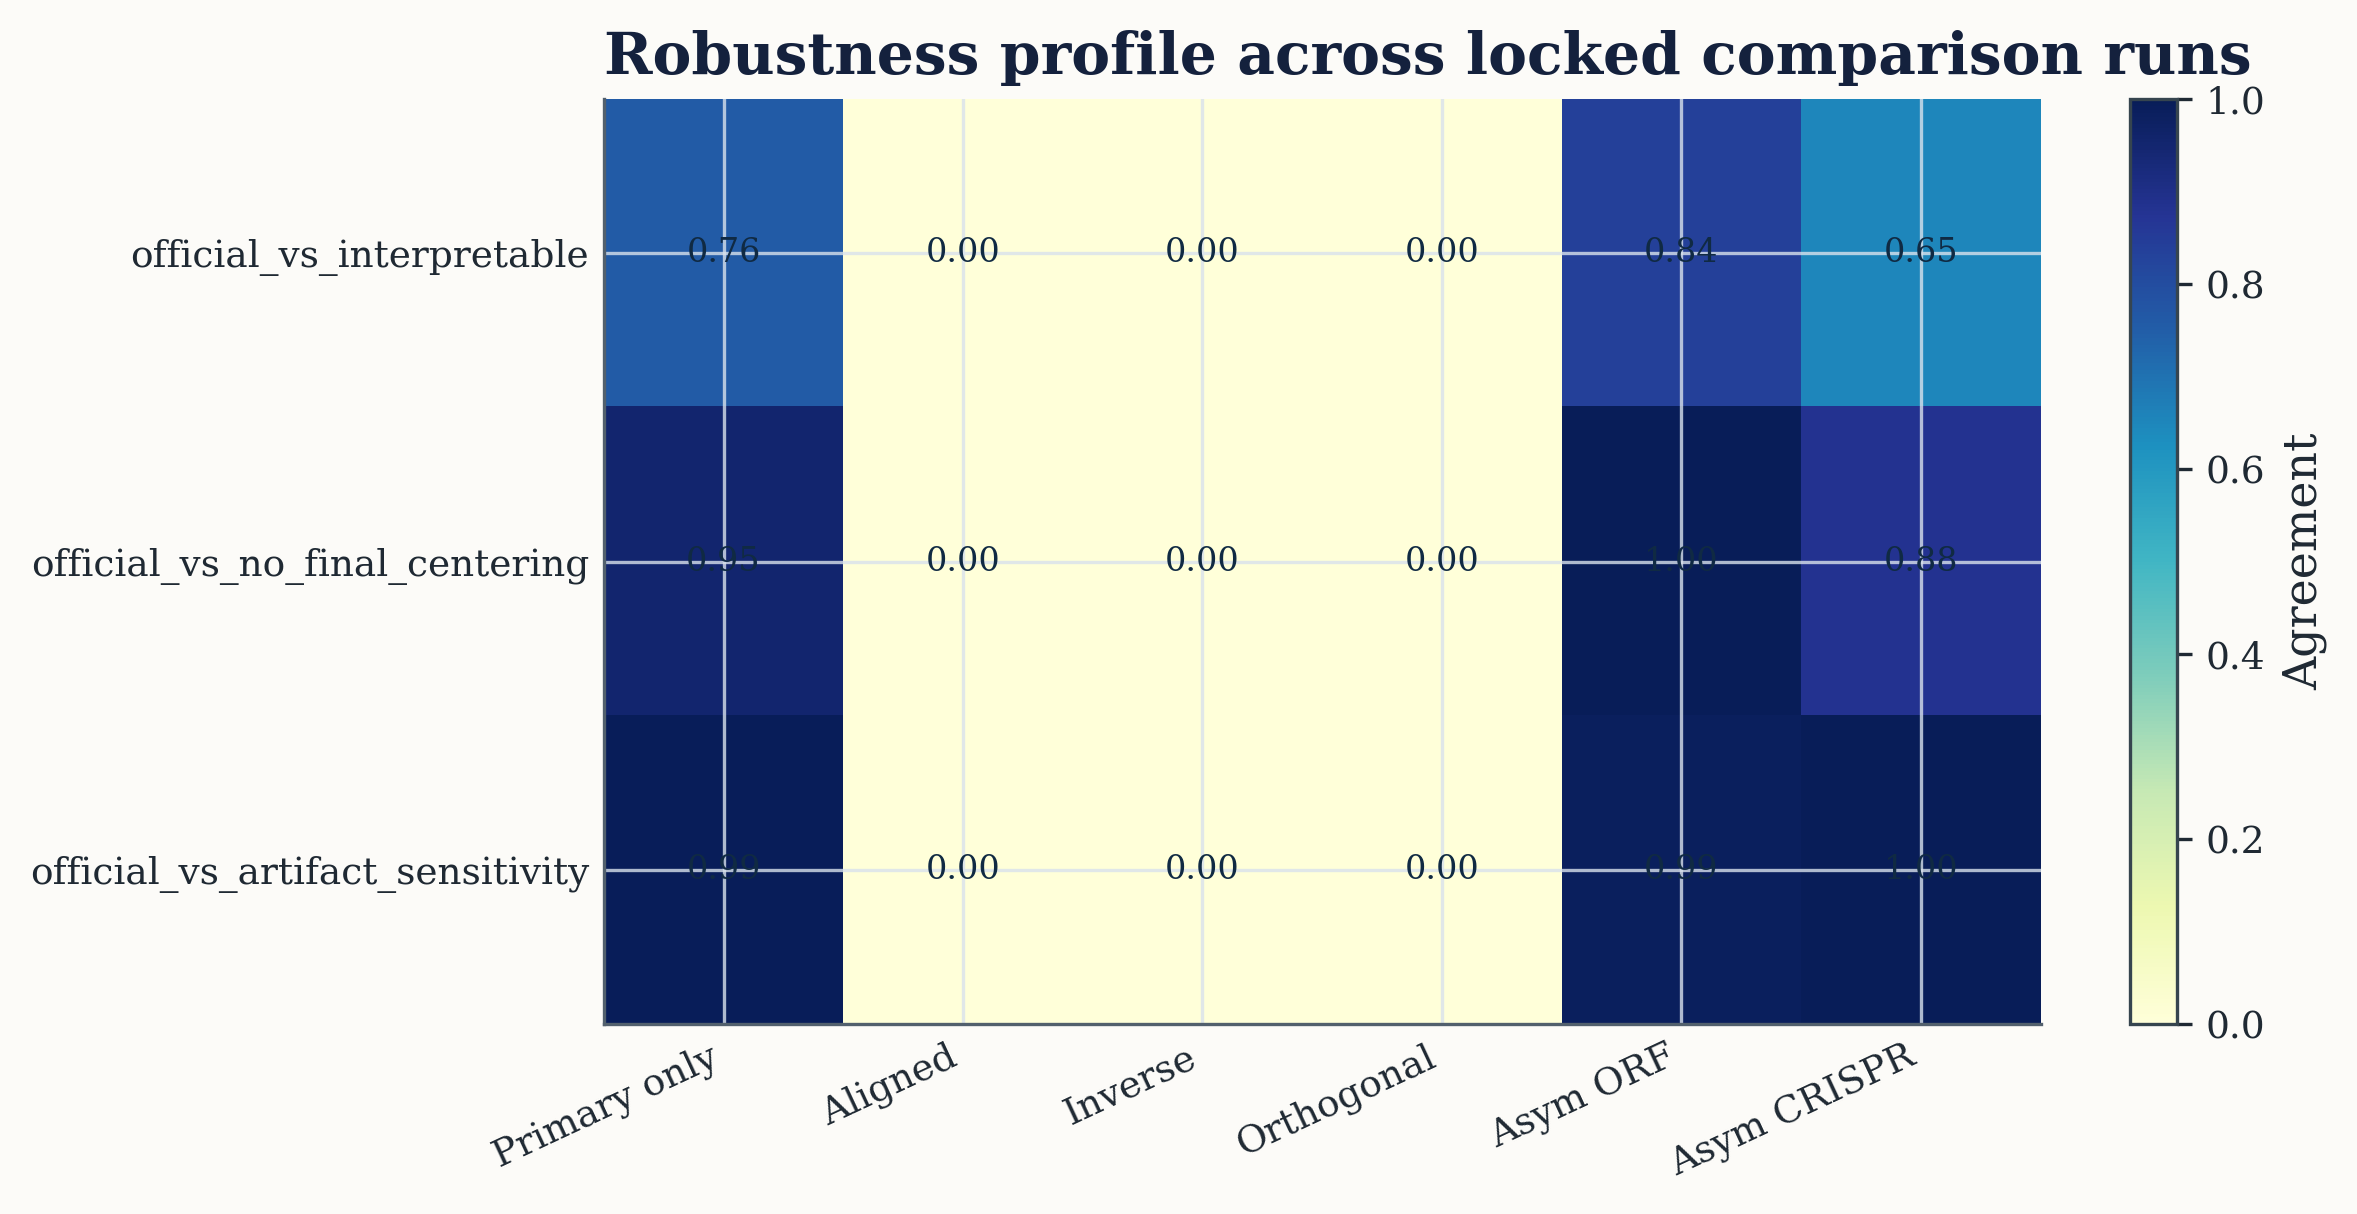
\includegraphics[width=0.93\textwidth]{figure3_stability.png}
\caption{\textbf{Robustness is uneven rather than absent.} Agreement remains high for no-final-centering and artifact sensitivity, but drops under the interpretable pipeline, supporting a fragility narrative rather than a uniformly stable positive one.}
\end{figure}

\begin{figure}[H]
\centering
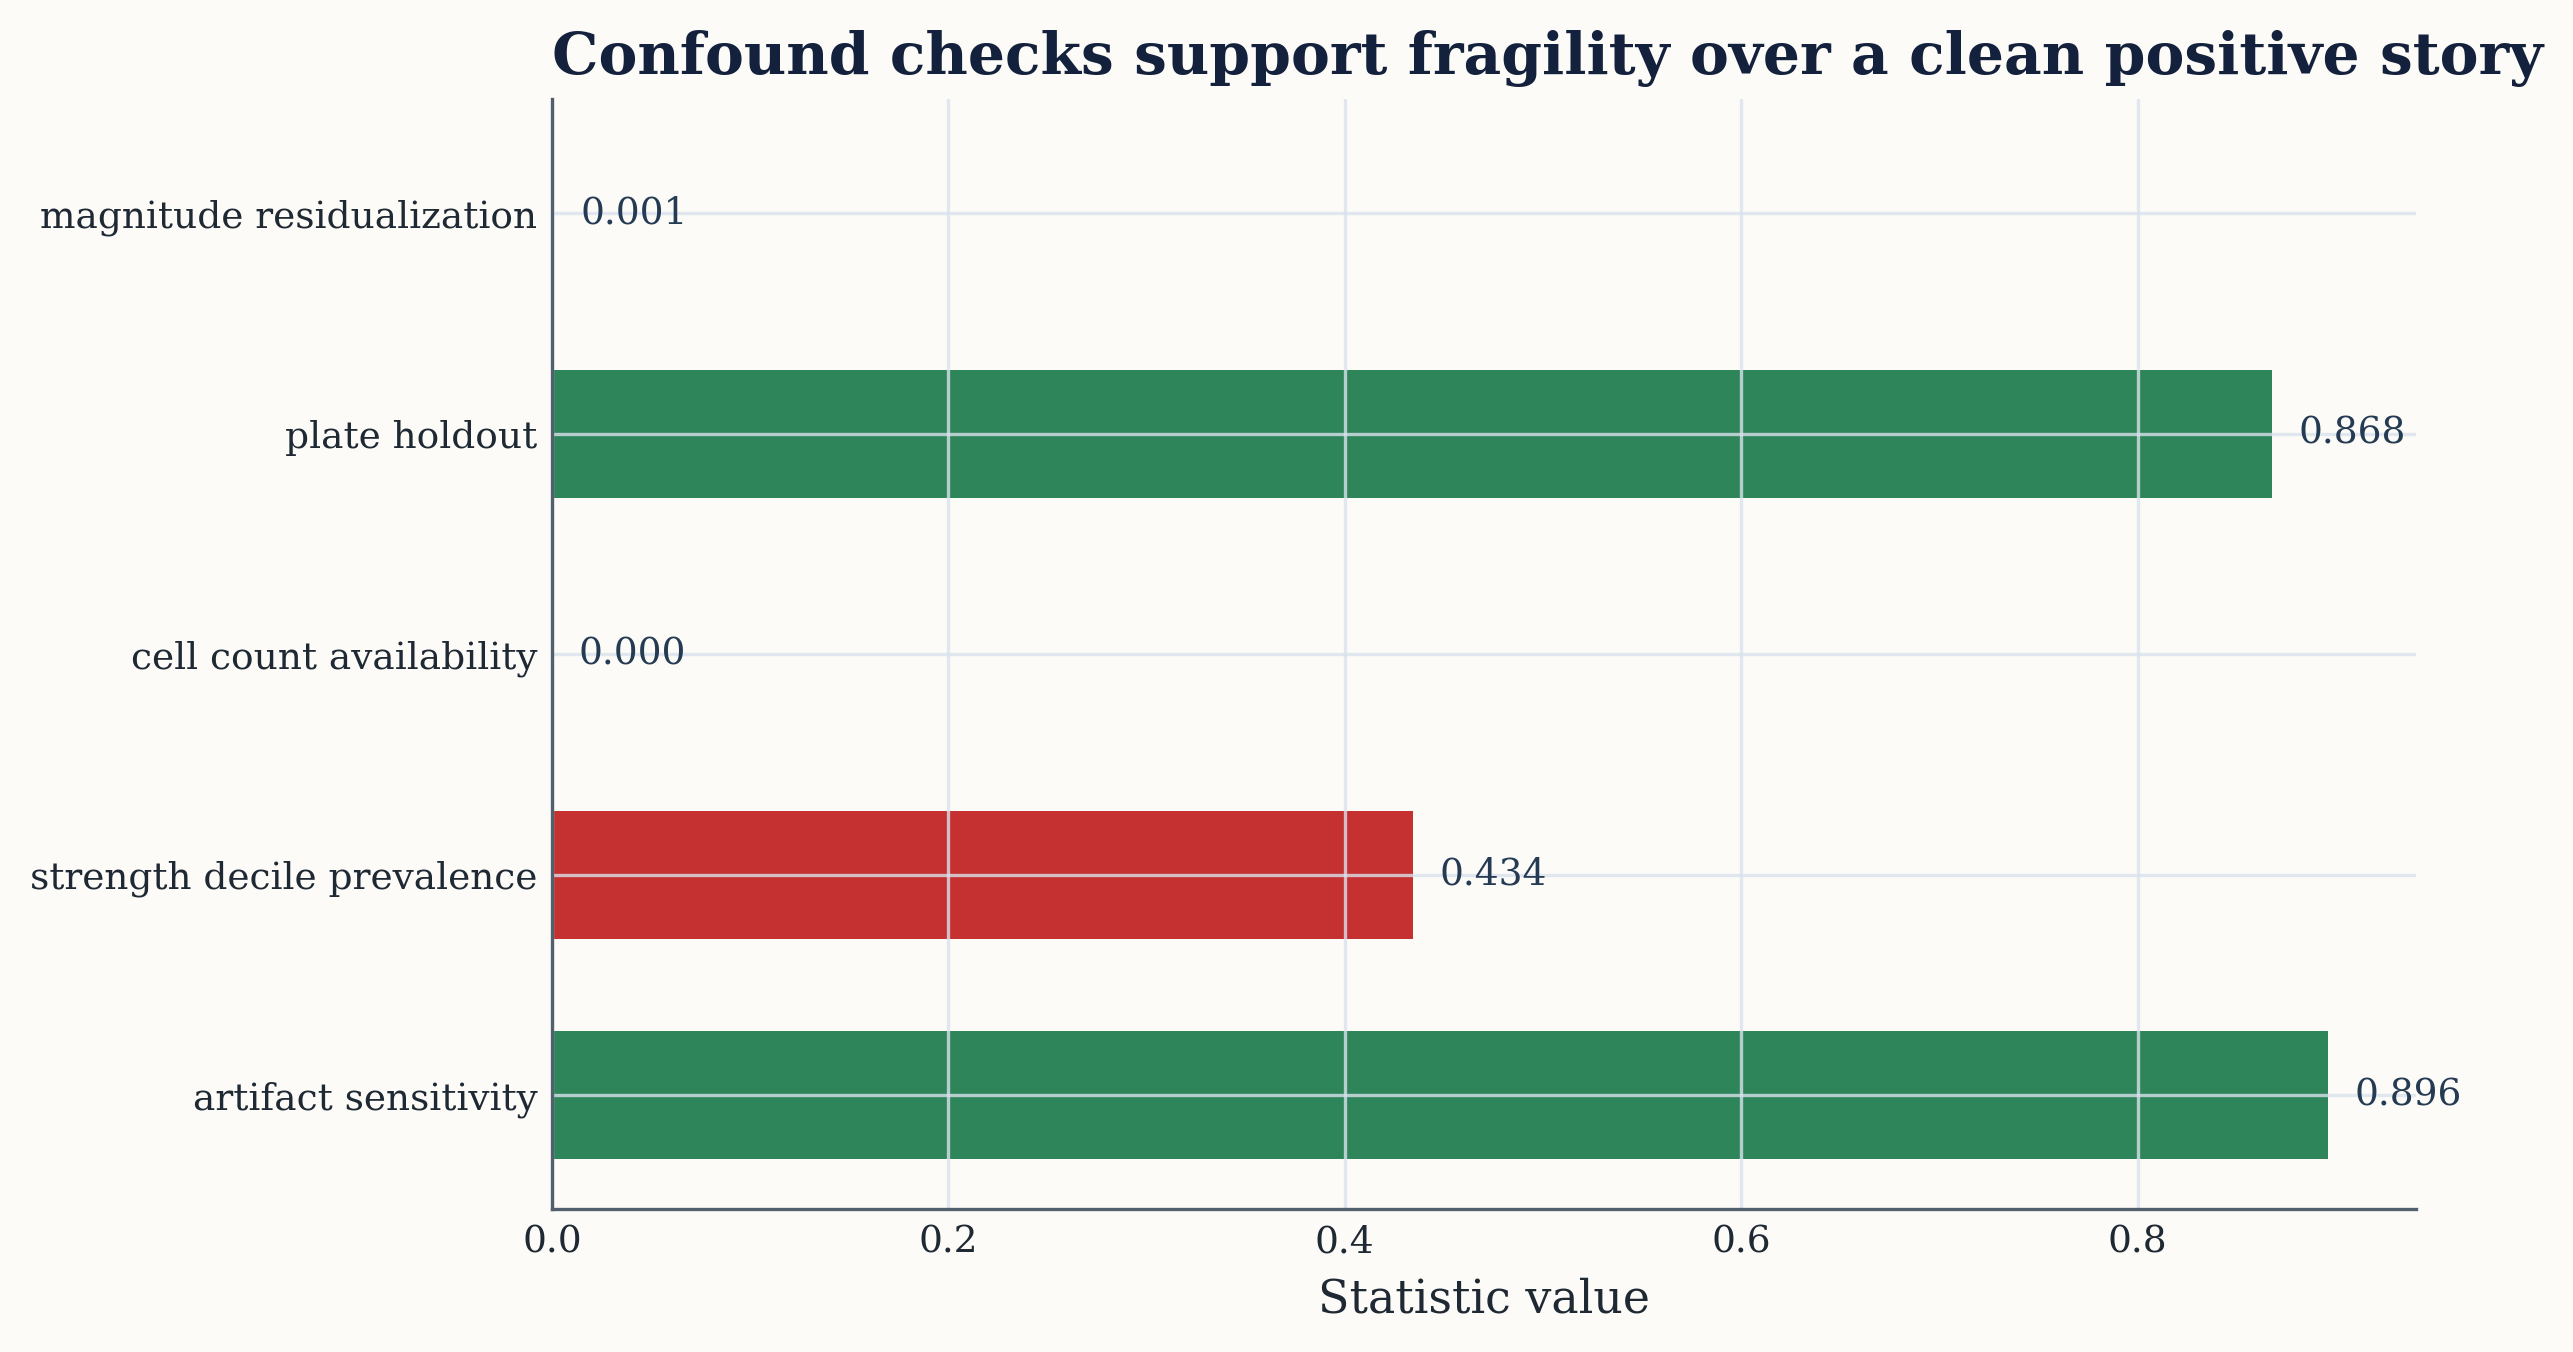
\includegraphics[width=0.93\textwidth]{figure6_confounds.png}
\caption{\textbf{Confound checks support a fragility interpretation.} Plate holdout and artifact sensitivity are reassuring, but strength-decile prevalence shift remains the explicit reason the final paper framing pivots away from a strong positive story.}
\end{figure}

\subsection{Biological enrichment survives, especially in asymmetric regimes}
Despite the fragility story, the regime map is not biologically empty. The official run produced 536 significant Reactome terms and high canonical-symbol coverage, with the strongest enrichment concentrated in asymmetric regimes. The top terms emphasize RNA metabolism, viral infection pathways, DNA repair, cellular stress responses, and pre-mRNA processing. These are not arbitrary categories, and their recurrence across asymmetric\_CRISPR and asymmetric\_ORF regimes supports the view that the regime map reflects real underlying biology rather than pure noise.

The asymmetry of the enrichment story is itself informative. Rather than showing a broad symmetric inversion between ORF and CRISPR, the map suggests that morphology often responds to the same gene in one direction more cleanly than in the other. That observation is compatible with dosage sensitivity, buffering, incomplete knockout efficiency, ORF overexpression artifacts, or pathway nonlinearities. The present paper cannot adjudicate among those mechanisms, but it does show that the morphology space is organized enough to surface them.

\begin{figure}[H]
\centering
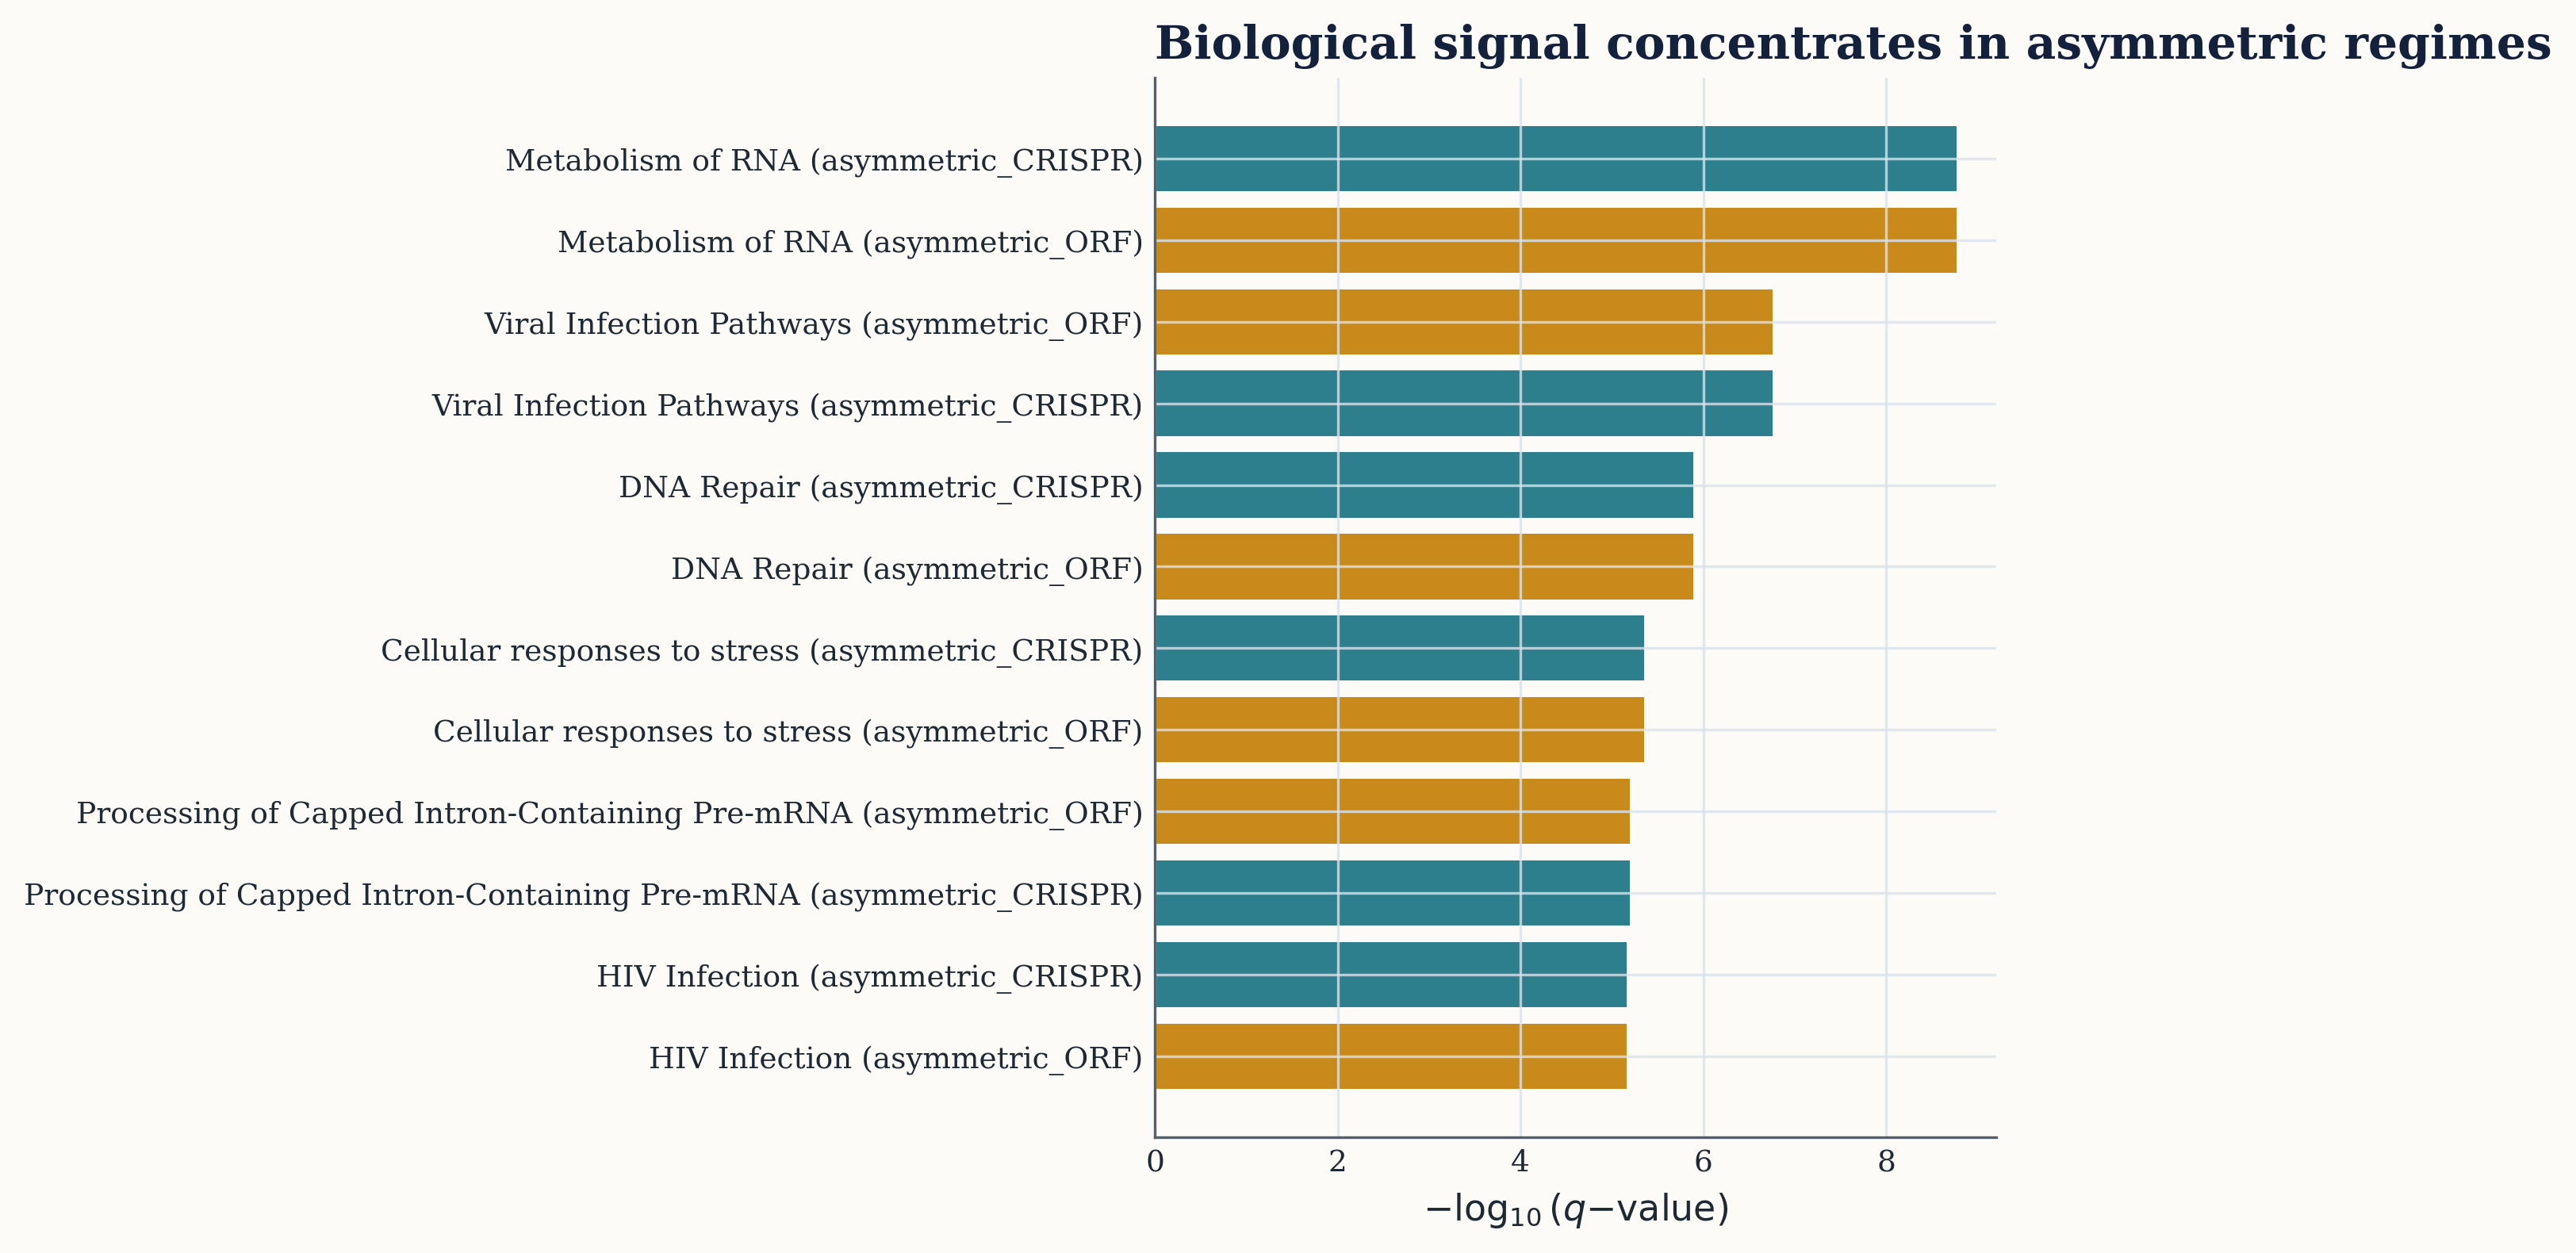
\includegraphics[width=0.93\textwidth]{figure5_enrichment.png}
\caption{\textbf{Biological structure is present even though the global framing is negative.} Significant Reactome signal concentrates in asymmetric regimes, reinforcing that the main result is not ``no biology,'' but ``biology that does not resolve into a robust symmetric geometry.''}
\end{figure}

\subsection{Retrieval does not support a discovery-style predictive claim}
The weakest part of the original hypothesis is retrieval. The regime-aware primary score reached an official MRR of only 0.001656, with essentially negligible hits@1. Competing scores were similarly poor. The interpretable pipeline did not rescue the situation; in fact, its signed and absolute cosine retrieval metrics slightly exceeded its primary regime-aware score. In practical terms, the geometry does not function as a useful same-gene retrieval engine.

This matters because retrieval would have been the natural way to convert a descriptive regime map into a stronger predictive claim. Without it, the signed regime representation cannot credibly be presented as an especially useful operational score. The more defensible interpretation is therefore descriptive and diagnostic rather than predictive.

\begin{figure}[H]
\centering
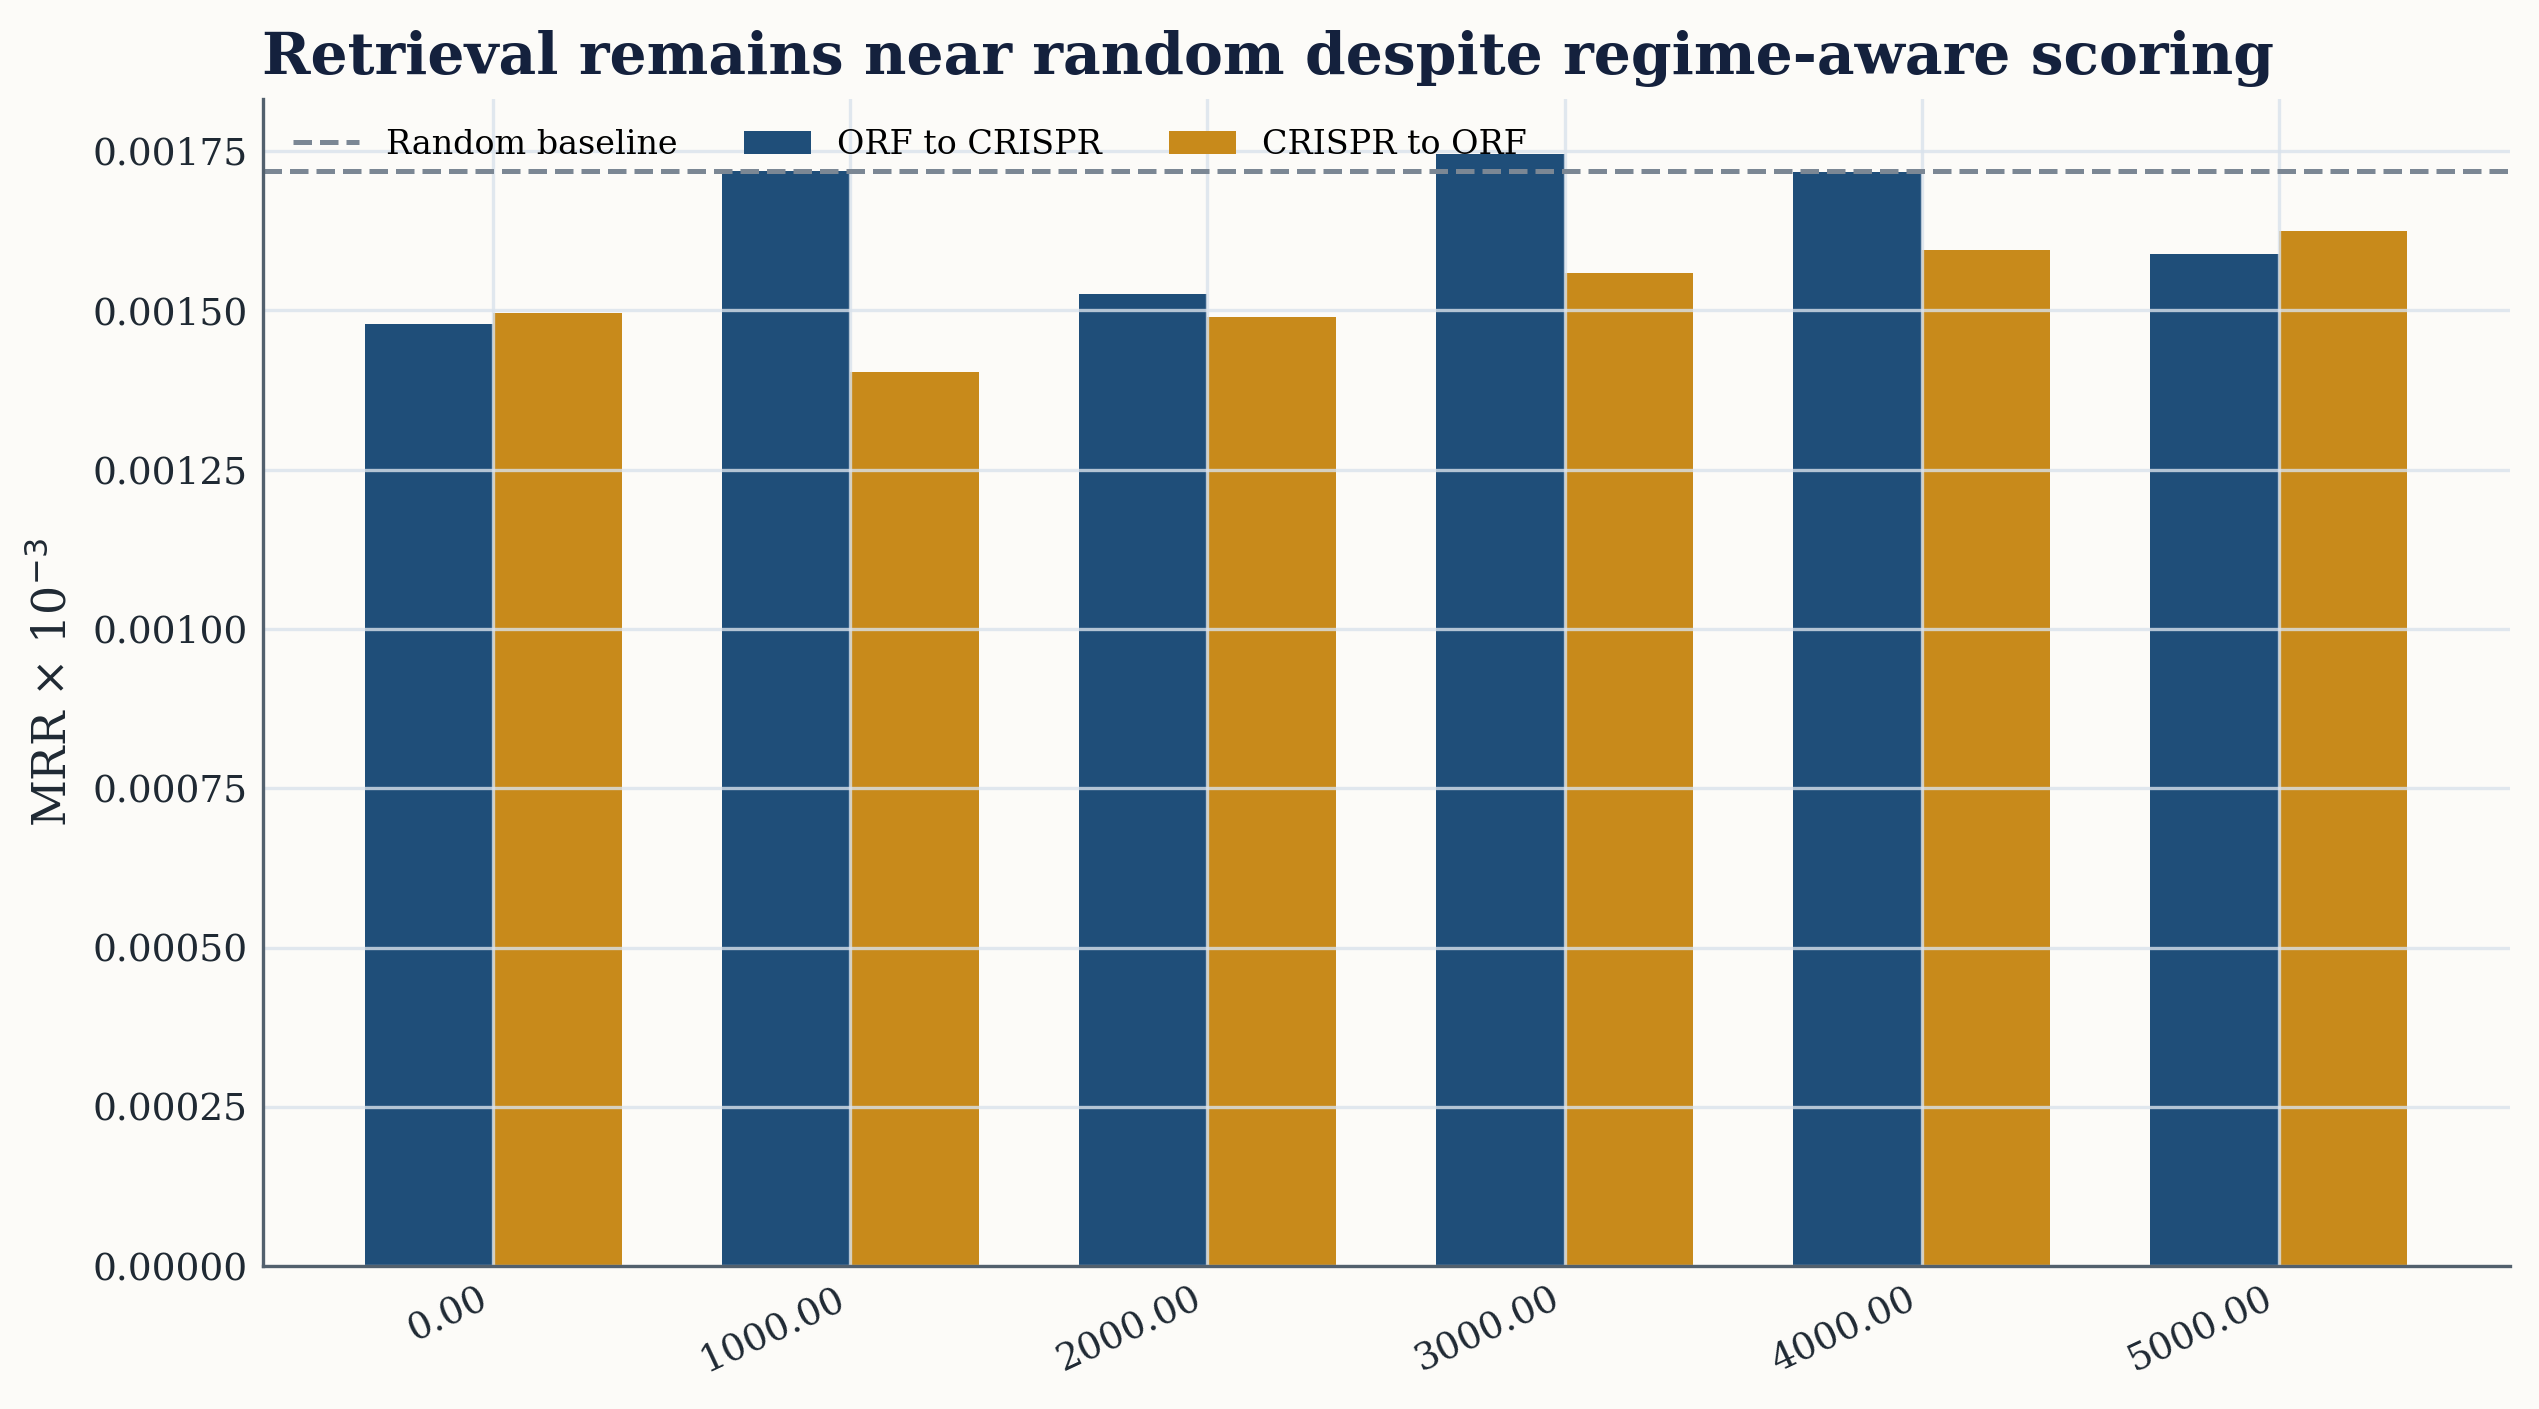
\includegraphics[width=0.93\textwidth]{figure4_retrieval.png}
\caption{\textbf{Retrieval remains close to random.} The geometry-derived score does not separate itself from other weak baselines strongly enough to support a utility-forward claim.}
\end{figure}

\section{Discussion}
The evidence supports a restrained interpretation of signed intervention geometry rather than a discovery-style claim. This interpretation has three parts.

First, there \emph{is} a same-gene morphological structure. The result is not a null in the trivial sense. The official run has thousands of active same-gene pairs, a large confident non-inactive subset, and substantial biological enrichment. Second, that structure is overwhelmingly asymmetric and ambiguous. The absence of surviving aligned, inverse, and orthogonal final labels is the clearest sign that the intuitive ``signed geometry'' story is too clean for the evidence. Third, the robustness pattern is mixed enough that fragility becomes the scientifically responsible headline. The map is highly stable to some perturbations, only moderately stable to others, and explicitly flagged by a strength-related confound.

That combination suggests a more interesting message than simple failure. Morphological correspondence between gain- and loss-of-function perturbations appears to be real but non-universal, mediated by regime-specific asymmetry, and highly sensitive to how effect size interacts with the preprocessing stack. In that sense, the study is less about proving a law than about defining a boundary: what kinds of morphology-derived same-gene structure can be defended under a locked pipeline, and what kinds cannot.

For readers working in image-based profiling, this is a useful result. Many morphology papers are vulnerable to silent analytic flexibility, especially when the underlying biology is complex and the signals are subtle. A paper showing that even large, high-quality public perturbation resources yield a \emph{fragile} regime geometry under locked conditions is therefore methodologically valuable. The result warns against overclaiming while still preserving genuine biological content.

\section{Limitations}
This study has four central limitations. First, it is scoped to the \texttt{cpg0016} resource and should not be generalized beyond this dataset without caution. Second, the regime taxonomy is descriptive rather than mechanistic; the paper cannot distinguish whether asymmetry is driven by dosage, editing efficiency, pathway nonlinearity, or residual technical artifacts. Third, there is no wet-lab validation. Fourth, the retrieval result is too weak to support an operational-usefulness claim, which narrows the scientific contribution to descriptive structure and fragility rather than prediction.

\section{Conclusion}
Under a locked analysis of matched ORF and CRISPR Cell Painting profiles, same-gene perturbations do not support a clean, robust signed-geometry discovery claim. They do, however, reveal a biologically structured and predominantly asymmetric landscape whose fragility is itself reproducible and scientifically informative. The resulting contribution is a cautionary but constructive boundary for the literature on high-dimensional image-based perturbation profiling: structured morphology is present, yet strong symmetric-geometry and retrieval-forward claims do not survive locked robustness scrutiny.

\begin{table}[H]
\centering
\caption{\textbf{Claim-level interpretation of the locked evidence bundle.} Each claim is retained or rejected according to the completed official and comparison runs.}
\begin{tabularx}{\textwidth}{>{\raggedright\arraybackslash}p{0.10\textwidth} >{\raggedright\arraybackslash}p{0.20\textwidth} >{\raggedright\arraybackslash}X}
\toprule
Claim & Status & Interpretation \\
\midrule
C1 & Positive & A real same-gene morphological regime structure exists. \\
C2 & Fragility & The structure is partially stable but not robust enough for a uniformly positive story. \\
C3 & Positive & Biological enrichment is present, especially in asymmetric regimes. \\
C4 & Unsupported & Retrieval is too weak to support a utility-forward or predictive framing. \\
\bottomrule
\end{tabularx}
\end{table}

\section*{Data and Code Availability}
All figures, source data, paper assets, and release artifacts referenced here were generated from the locked official run directory for \texttt{offv1\_\_featint\_\_platectrl\_\_thrA2\_thrR2\_\_z1p96\_\_beta1p0}. This root-level manuscript folder is a convenience copy of that finalized paper package. The manuscript should therefore be interpreted together with the completed run bundle and its corresponding \texttt{claim\_evidence\_matrix.csv}, \texttt{pipeline\_agreement.csv}, \texttt{confound\_summary.csv}, and \texttt{release\_report.json} artifacts.

\begin{thebibliography}{9}

\bibitem{bray2016cellpainting}
Bray, M.-A., Singh, S., Han, H., Davis, C. T., Borgeson, B., Hartland, C.,
Kost-Alimova, M., Gustafsdottir, S. M., Gibson, C. C. \& Carpenter, A. E.
\newblock Cell Painting, a high-content image-based assay for morphological profiling using multiplexed fluorescent dyes.
\newblock \emph{Nature Protocols} \textbf{11}, 1757--1774 (2016).
\newblock \url{https://doi.org/10.1038/nprot.2016.105}

\bibitem{cimini2023optimizing}
Cimini, B. A. et al.
\newblock Optimizing the Cell Painting assay for image-based profiling.
\newblock \emph{Nature Protocols} \textbf{18}, 1981--2013 (2023).
\newblock \url{https://doi.org/10.1038/s41596-023-00840-9}

\bibitem{jump2025genetic}
Chandrasekaran, S. N. et al.
\newblock Morphological map of under- and overexpression of genes in human cells.
\newblock \emph{Nature Methods} \textbf{22}, 1742--1752 (2025).
\newblock \url{https://doi.org/10.1038/s41592-025-02753-9}

\bibitem{chandrasekaran2021upgrade}
Chandrasekaran, S. N., Ceulemans, H., Boyd, J. D. \& Carpenter, A. E.
\newblock Image-based profiling for drug discovery: due for a machine-learning upgrade?
\newblock \emph{Nature Reviews Drug Discovery} \textbf{20}, 145--159 (2021).
\newblock \url{https://doi.org/10.1038/s41573-020-00117-w}

\bibitem{way2022complementary}
Way, G. P. et al.
\newblock Morphology and gene expression profiling provide complementary information for mapping cell state.
\newblock \emph{Cell Systems} \textbf{13}, 911--923.e9 (2022).
\newblock \url{https://doi.org/10.1016/j.cels.2022.10.001}

\end{thebibliography}

\end{document}
